% DOC SETTINGS ===================================
\documentclass{article}
\usepackage[utf8]{inputenc}
\usepackage{fancyhdr}
\pagestyle{fancy}
\usepackage{geometry}
 \geometry{
 a4paper,
 total={170mm,257mm},
 left=20mm,
 top=25mm,
 }
\fancyheadoffset{0mm}
\lhead{ECE4540 HW0}
\rhead{Kavin Thirukonda 2021}
\usepackage{steinmetz}
\usepackage{listings}
\usepackage{circuitikz}
\usepackage{wrapfig}
\usepackage{mathtools}  
\usepackage[font=small]{caption}
\mathtoolsset{showonlyrefs} 
\cfoot{}
% DOC SETTINGS ===================================
\begin{document}
\section*{Abstract}

The focus of this paper is to show the outlook of the semiconductor industry in terms of the companies and how someone working in the industry can expect certain quality of life factors to be. It very clear that the semiconductor industry is under growth and has been since the birth of semiconductors, there is no alternative so there is no slowing down. Someone working in the industry get highly paid compared to other fields because of the job demand. From those two factors alone it is clear that working in the industry is a good option.
\section*{Findings}
\subsection*{Top Players and Driving Factors}
\begin{wrapfigure}[17]{r}{.5\textwidth}
  \begin{center}
    \boxed{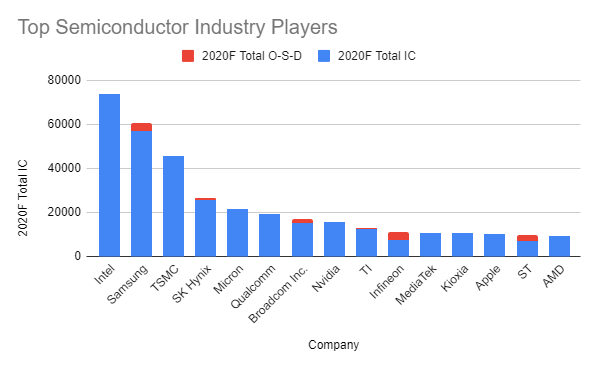
\includegraphics[width=0.45\textwidth]{top_players.png}}
  \end{center}
  \caption{Top 15 Players}
\end{wrapfigure}
Knowing who the top players in the industry are is important as they will have the most capital and will most likely be using the most cutting edge technology. The bar graph in figure one shows the top 15 players in the semiconductor industry, with IC values separated from OSC giving a total look at who has the most involvement. This list includes both foundries, fabless, and standard companies. As can be seen, Intel is the top company with 73,894 semiconductors coming out of production with a nontrivial gap between them and their closest competitor.

It is important to consider what are the driving factors in the semiconductor industry. Knowing what these factors are can be good for when the factors are gone. One clear correlation that anyone can see is consumer electronic demand, this showed itself in full swing during the pandemic in relation to the chip shortage. While production lines being stopped due to the pandemic is certainly a problem, one of the main reason that the IC shortage occurred is because demand rapidly increased for home computers and devices as people started to more frequently work from home. From that we can see that as long as no alternative for semiconductor IC's exist and there is an electronic device demand, the semiconductor industry will continue to grow.

It is worth noting that the top players in the semiconductor industry have stayed relatively consistent since its conception, for example Intel was one of the first companies to create semiconductor products and today it remains the top producer, which means general job security would be very good. Another way to see whether or not working in the semiconductor industry would have good job security would be to look at the growth over the past years and the projections for what they will become. 


\subsection*{Job Growth And Compensation}
\begin{wrapfigure}{l}{.5\textwidth}
  \begin{center}
    \boxed{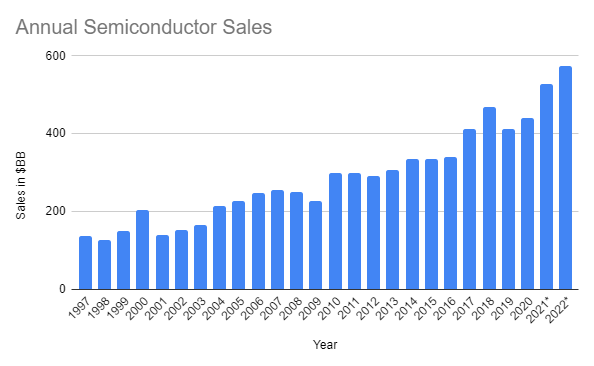
\includegraphics[width=0.45\textwidth]{annual_sales.png}}
  \end{center}
  \caption{Annual Sales}
\end{wrapfigure}
With the world becoming more and more digital and no replacement for semiconductor based transistors in sight, the growth for the semiconductor is all but guaranteed. One way to see this is with annual semiconductor sales, which can be seen in figure two. As can be seen in the figure, there has been a gradual but steady increase in the annual sales of semiconductor products even as early as 1997. There is also projected values for the end of 2021 as well as the projected value for 2022. This is no surprise since there is no alternative to semiconductor technology that boasts the same size, speed, and power benefits.

Even with good job growth there needs to be good benefits for working in the field for pursuing the job to be a good option, so it is always good to look at salary metrics for a VSLI/IC designed as this is the main factor that people look at when thinking about getting a job.

\newpage

\begin{wrapfigure}{l}{.5\textwidth}
  \begin{center}
    \boxed{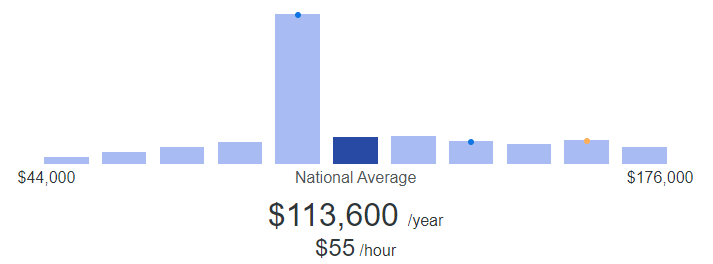
\includegraphics[width=0.45\textwidth]{wage.png}}
  \end{center}
  \caption{Salary information}
\end{wrapfigure}

According to salary.com the average salary for a VLSI/IC designer is 113,600 per year averaging across all locations. this values is certainly above average compared to most jobs in the computer engineering fields. As stated before the average salary is based on all locations, so it is useful to see what the average salary is for somewhere like silicon valley in California, which is obviously called silicon valley for a reason. In San Francisco the average VSLI/IC designer salary is 145,657 per year. This is a significant step up, but the housing market must also be considered in this metric.

It  can also be seen that depending on where you live and how many years of experience you have it is not totally uncommon to make up to 200,000 a year which is a good reason to be staying in the industry long term.
\subsection*{Hiring Demographics}
\begin{wrapfigure}{r}{.5\textwidth}
  \begin{center}
    \boxed{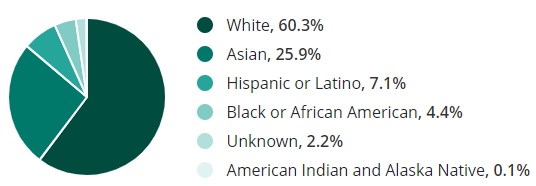
\includegraphics[width=0.45\textwidth]{race.png}}
  \end{center}
  \caption{Race Demographics}
\end{wrapfigure}
For people who care about diversity in the work place, knowing the hiring demographics is important to be aware of, while not all that much information exist about the demographics of specifically VSLI/IC designers there is some information about ASIC designers which I presume most of the information would be relatively uniform across the two professions.  

From figure four we can see that like every field in America, the main contenders are white Americans, with Asian, and Hispanic Americans behind them. From personal experience I think this will be something that changes very soon. In the internship that I have participated in the majority of white Americans who do work these jobs are very old, and all younger employees have a very good spectrum of diversity to them. So if the lack of diversity is a problem for someone, it would be good to know that it has a chance to be changing soon.

\begin{wrapfigure}{l}{.4\textwidth}
  \begin{center}
    \boxed{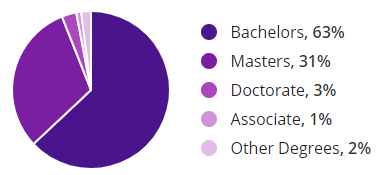
\includegraphics[width=0.35\textwidth]{degree.png}}
  \end{center}
  \caption{Degree Requirements}
\end{wrapfigure}
Along with diversity, it would good to know if one would need to go to grad school to get a good job in 
VLSI/IC design, in figure five we can see that the vast majority don't have grad school degrees, but at the same time there is a good chunk of people who do. And as a general rule of thumb having a graduate degree is a sure fire way to get paid more.

Another thing to note is that bachelor degrees have the majority, but also associate degrees have almost no representation, so from that we can see that going to a four year university is essentially a must to be a VSLI/IC designer or you probably wont even get a job in the field. This would make sense as learning all the curriculum needed to operate efficiently in the field would be hard in only two years.


\section*{Sources}
\begin{itemize}
\item https://www.netscribes.com/semiconductor-industry-trends/
\item https://www.salary.com/research/salary/recruiting/vlsi-design-engineer-salary
\item https://www.icinsights.com/news/bulletins/Intel-To-Keep-Its-Number-One-Semiconductor-Supplier-Ranking-In-2020/
\item https://www.statista.com/statistics/266973/global-semiconductor-sales-since-1988/
\item https://www.ziprecruiter.com/Salaries/VLSI-Engineer-Salary
\end{itemize}
\end{document}
